\section{Method: A Structure-Aware Hybrid Estimator}

\subsection{Classifying Every Neuron as Dead, Kink, or On Before Any Sampling}

Before choosing an algorithm, we selected a few example MLPs and drew a large number of Monte Carlo samples to visualize the pre-activation distribution for each neuron under Gaussian inputs. We noticed that, particularly for the middle and later layers of the MLP, there were many pre-activation distributions with almost all probability mass below zero, some with substantial probability mass near zero, and others with almost all probability mass above zero. These are the empirical dead, kink, and on regimes in \Cref{fig:layer-collapse-classification}.

By using the weights of the MLP to predict each neuron's regime prior to any sampling, we can create a white-box estimator that leverages the classical observation that rectifiers produce sparse active sets \citep{nair2010rectified,glorot2011deep}. Suppose the previous post-ReLU activations have approximate mean $\mu_{\ell-1}$ and diagonal variance $v_{\ell-1}$. For a column $j$ of $W_\ell$, the preactivation moments are approximated by

\begin{align}
    \mu_{\ell,j}^{\rm pre} &= \sum_i W_{\ell,ij}\mu_{\ell-1,i}, \label{eq:pre-mean}\\
    (\sigma_{\ell,j}^{\rm pre})^2 &= \sum_i W_{\ell,ij}^2 v_{\ell-1,i}. \label{eq:pre-var}
\end{align}
Writing $\alpha_{\ell,j}=\mu_{\ell,j}^{\rm pre}/\sigma_{\ell,j}^{\rm pre}$ and denoting the standard normal density and CDF by $\phi$ and $\Phi$, the Gaussian ReLU moment update is
\begin{align}
    \mu_{\ell,j}
    &= \mu_{\ell,j}^{\rm pre}\Phi(\alpha_{\ell,j})
       + \sigma_{\ell,j}^{\rm pre}\phi(\alpha_{\ell,j}), \label{eq:post-mean}\\
    v_{\ell,j}
    &= \left((\sigma_{\ell,j}^{\rm pre})^2+(\mu_{\ell,j}^{\rm pre})^2\right)\Phi(\alpha_{\ell,j})
       + \mu_{\ell,j}^{\rm pre}\sigma_{\ell,j}^{\rm pre}\phi(\alpha_{\ell,j})
       - \mu_{\ell,j}^2. \label{eq:post-var}
\end{align}

These are the same closed-form ReLU Gaussian moments used in assumed-density filtering for Bayesian neural networks \citep{hernandez2015probabilistic, ghosh2016adf}. The Gaussian assumption here is only an approximation, not an accurate representation of ReLU activations, especially in the later layers. Under Gaussian weight priors, unit-level pre- and post-activation marginals become increasingly heavy-tailed with depth and are characterized by sub-Weibull tails \citep{vladimirova2019understanding}. 

In this estimator, we use the normalized margin $\alpha_{\ell,j}$ to classify a neuron as dead if $\alpha<-3$, on if $\alpha>3$, and kink otherwise.

% \subsection{Empirical Difficulty Signal for Sample Allocation}

% When evaluating our estimator, we observed that the final-layer sampling variance is concentrated among a small subset of neurons. In a matched random MLP, the top $10\%$ of final neurons by mean magnitude carried about half of the expected final-layer sampling variance, and the top $20\%$ carried about $72\%$ (\Cref{fig:final-magnitude-sampling-difficulty}).

% \begin{figure}[t]
%     \centering
%     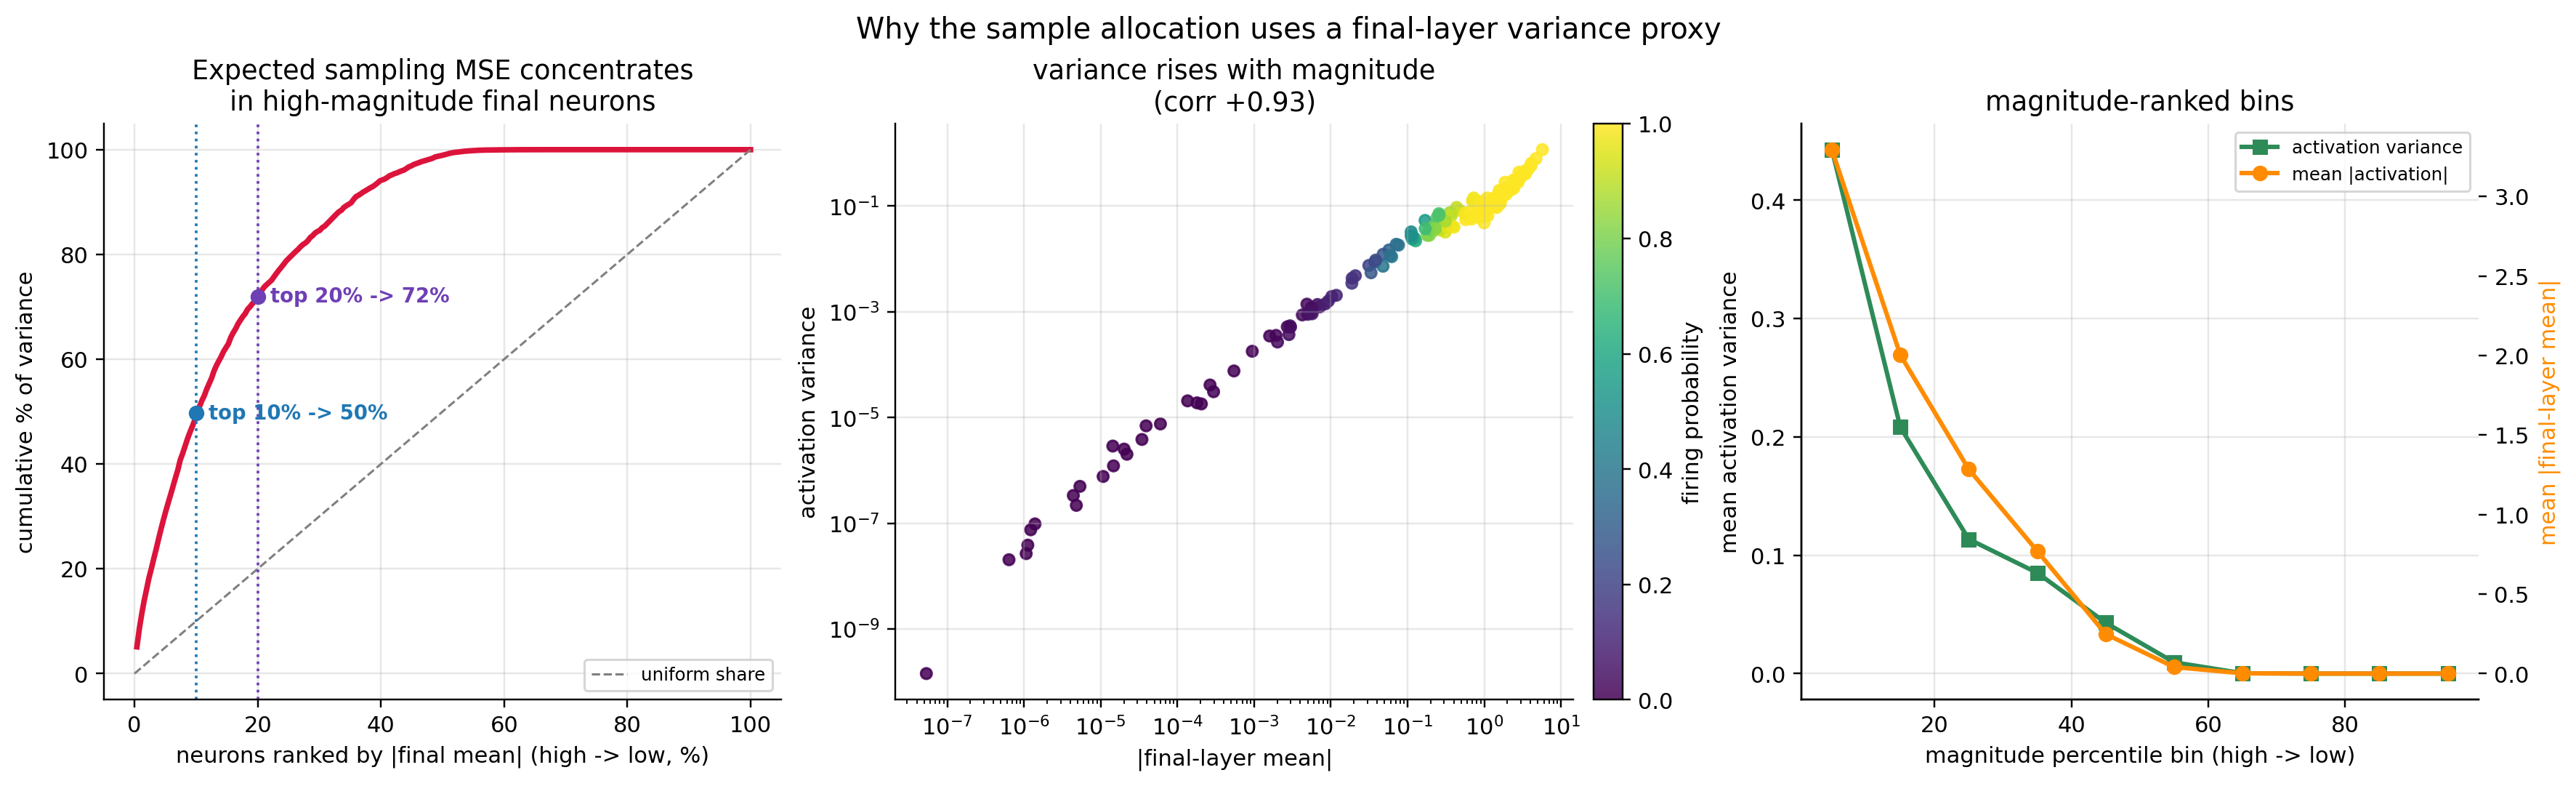
\includegraphics[width=\linewidth]{figures/final_magnitude_sampling_difficulty.png}
%     \caption{Empirical support for the sample-allocation proxy on a matched random ReLU MLP. Under plain Monte Carlo, each neuron's contribution to expected final-layer MSE is proportional to its activation variance divided by sample count. High-magnitude active final neurons carry most of this absolute sampling cost, so a final-layer variance proxy is a natural signal for allocating more samples to harder MLPs.}
%     \label{fig:final-magnitude-sampling-difficulty}
% \end{figure}

% Based on this finding, we decided to allocate samples strategically across MLPs, assigning more samples to MLPs whose final layers contain larger active, high-variance neurons according to the following rule:
% \begin{align}
%     N = \clip\left(2\cdot\mathrm{round}\left(\frac{49152}{2}\sqrt{\frac{\bar v_L}{0.02143}}\right),
%     30720,61440\right).
% \end{align}
% The allocation is intentionally smooth. Earlier bucketed or mini-tuned allocations produced local wins, but were less reliable on the public evaluator.

\subsubsection{What the Classification Buys: Skip the Dead, Sample the Kinks, Fold the On}

The regime model determines which sampled coordinates are materialized. Dead neurons do not need a sampled matmul column: their post-ReLU mean is either filled by the analytic pass or set to zero when the residual contribution is negligible. Kink neurons remain sampled, because their ReLU masks change across samples. On neurons are treated as linear in later layers. If neuron $i$ is on at layer 30, then sample by sample
\begin{align}
    x_{30,i}=z_{30,i}=(x_{29}W_{30})_i.
\end{align}
Its contribution to a layer-31 preactivation can therefore be composed through $W_{30}$ and $W_{31}$ without materializing the sampled layer-30 column. Layer-30 kink neurons do not satisfy this identity, so their contribution remains sampled.

One disadvantage of using a classifier is that the boundary between regimes is not always clear. To overcome this shortcoming, a small prefix sample is used to identify neurons near the decision boundary, which are reevaluated using a larger prefix sample before being reassigned if necessary. This verification is particularly important in layers 30 and 31, where classification errors directly affect the scored layer.

\subsection{Cold-Column Slicing: Skipping the Zero Blocks of the Sampled Activations Exactly}

\begin{figure}[p]
    \centering
    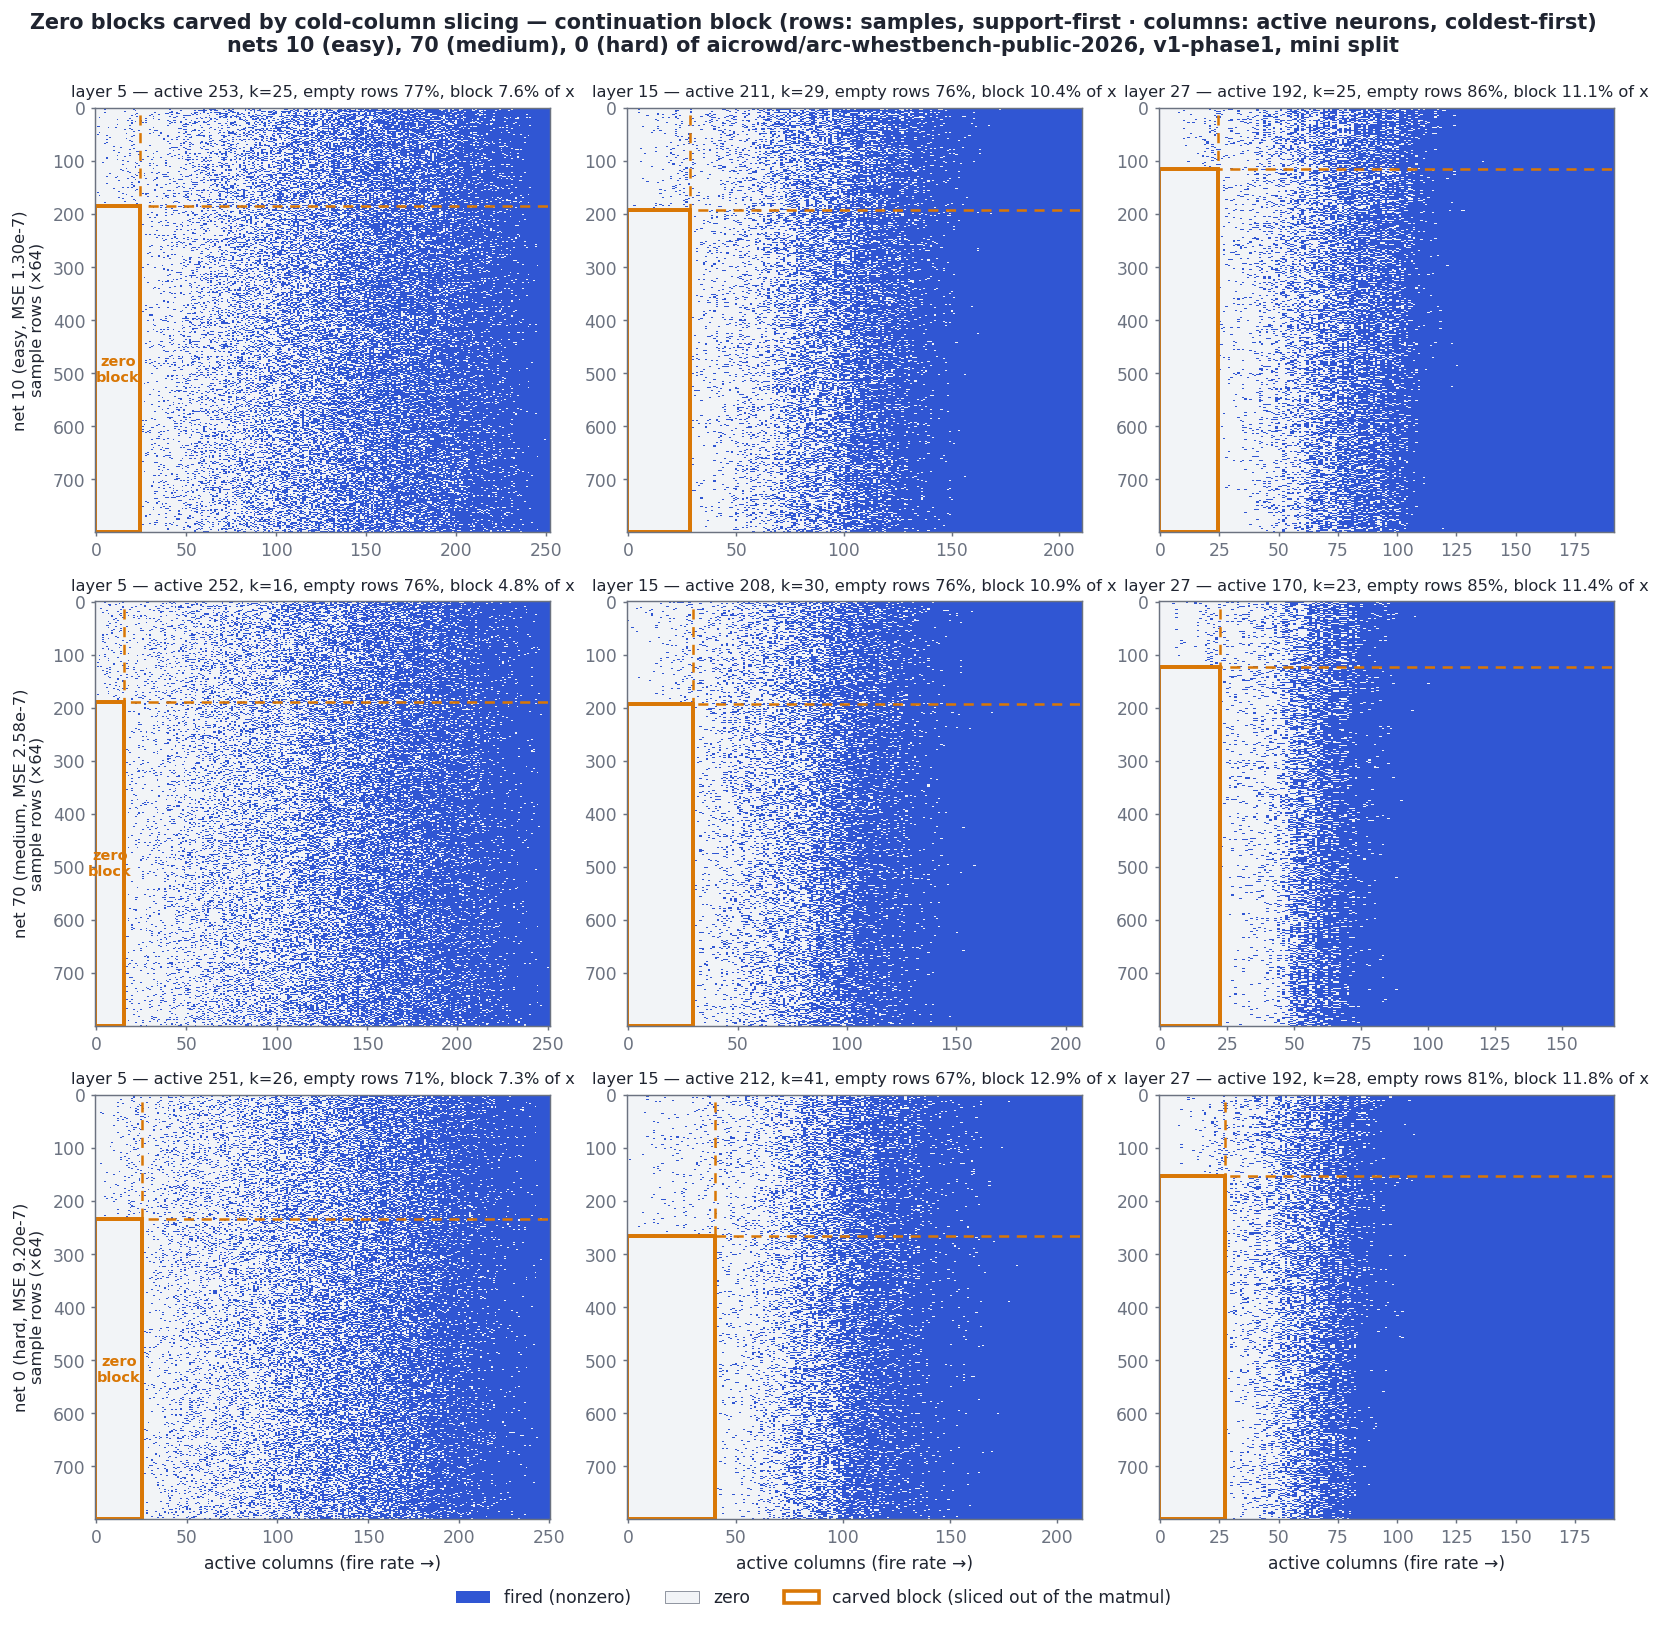
\includegraphics[width=\linewidth]{figures/coldslice_blocks.png}
    \caption{The zero blocks that cold-column slicing skips, captured from the shipped estimator's own continuation blocks (51{,}200 sample rows $\times$ active columns). Rows of the grid are three public mini networks of increasing difficulty (nets 10, 70, 0); grid columns are layers 5, 15, and 27. Within each panel, matrix columns are sorted coldest-first and sample rows are sorted so that rows firing on the cold set come first, exactly the order the estimator uses. The outlined bottom-left rectangle is the payoff: those rows never fire on those columns, so the block is all zero and the propagating matmul never touches it.}
    \label{fig:coldslice-blocks}
\end{figure}

The dead/kink/on split reduces compute primarily by removing the computation for dead neurons, but the sampled activations of the surviving neurons still contain many zeros. To see where they are, sort the columns of the sampled post-ReLU activation matrix by firing rate, the fraction of Monte Carlo samples on which each neuron is active. \Cref{fig:coldslice-blocks} shows the result across three networks and three depths. High-fire (``hot'') columns are dense. At the left edge of each panel sits a band of rarely-firing (``cold'') columns that is almost entirely zero, with only scattered firings.

Which of these zeros are worth skipping depends on the cost model. The challenge bills every gathered element, so evaluating the sparse product row by row with gathers costs more than the dense multiplication it replaces. Taking a contiguous slice of an array, on the other hand, is free. The estimator therefore only skips zeros where they form a contiguous rectangle that a slice can step around. About a third of the zeros are scattered through the hot block; they form no such rectangle, and we leave them alone.

\subsubsection{One Row Reorder Exposes a Zero Block the Matmul Can Skip}

The carve works layer by layer. First, the estimator decides which columns count as cold, using the firing rates measured during the pilot pass: the cold set is the $k$ active columns with fire rate below $0.03$, with $k$ clamped to $8 \le k \le 64$ and never allowed to shrink the hot block below 96 columns (below that width the Strassen routine stops paying off). Next, it arranges for those columns to arrive already sorted. This is free: reordering the previous layer's active-neuron list just changes which weight slice produces which output column, so the cold columns come out first without touching the data. Finally, one scatter reorders the sample rows so that every row that fires on at least one cold column (a ``support row'') comes first, and all the rows that never touch the cold set come after.

After this reordering, the bottom-left block of the matrix---the non-support rows crossed with the cold columns---is zero by construction (\Cref{fig:coldslice-blocks}). The product $XW$ then splits into two pieces: a hot-block multiplication over all rows, and a small correction multiplication over just the support rows and the cold columns. Because the rows and columns of each piece are contiguous, the correction is added onto a plain slice of the output; there are no gathers and no scatter-adds. The carve is also exact: it changes the route used to compute the sampled product, not the sampled estimator being evaluated.

\begin{figure}[t]
    \centering
    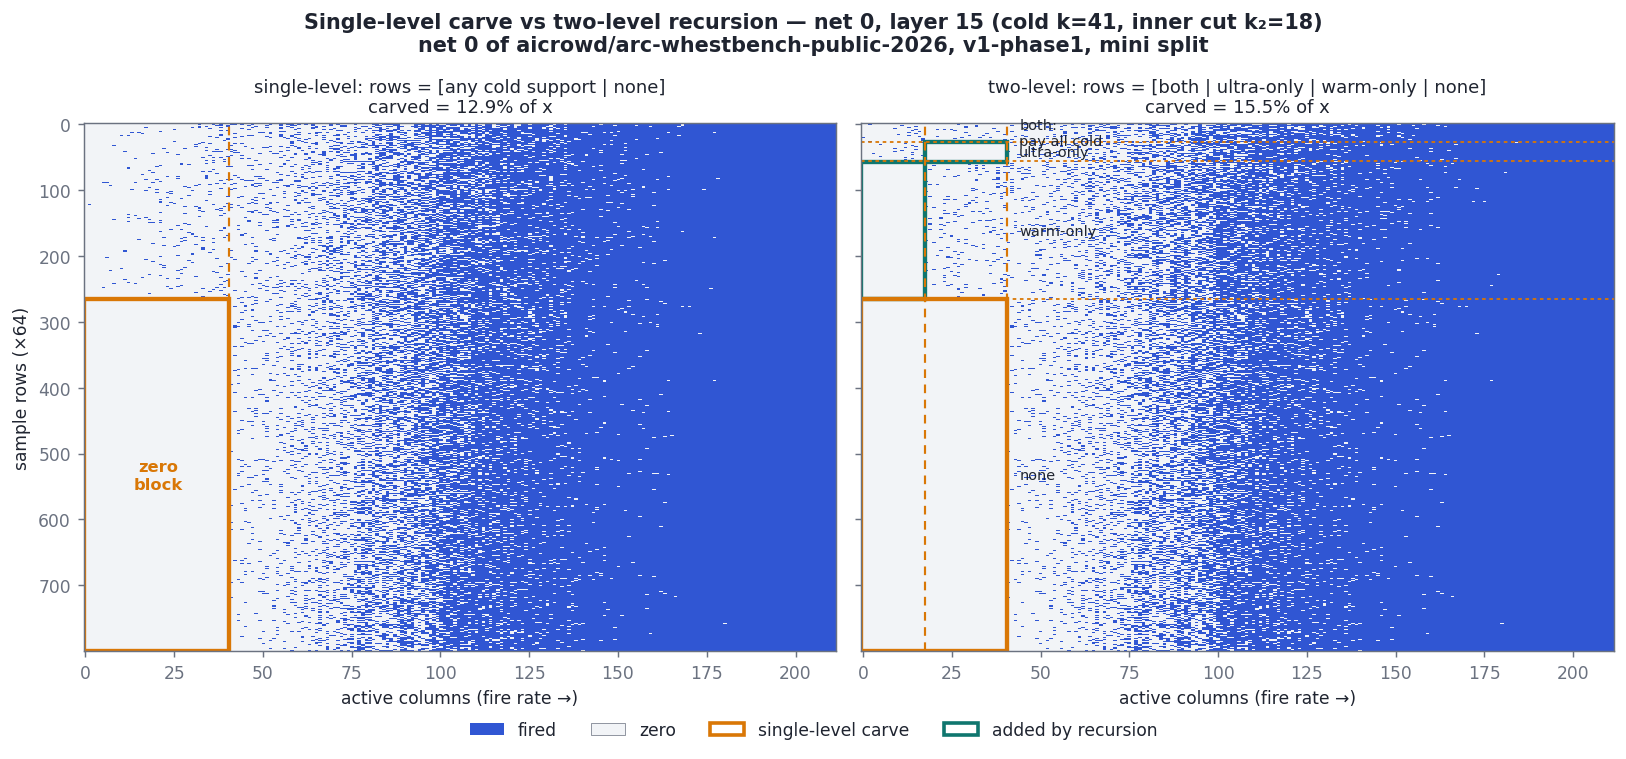
\includegraphics[width=\linewidth]{figures/coldslice_recursion.png}
    \caption{Single-level carve versus the two-level recursion, on the same continuation block (net 0, layer 15). Left: splitting rows only by ``fires on the cold set or not'' yields one zero rectangle. Right: splitting the cold set into ultra-cold and warm-cold slabs, and grouping rows by which slabs they fire on (both, ultra-only, warm-only, neither), turns one skipped rectangle into three. The added rectangles are zero by how the row groups are defined: an ultra-only row, for instance, by definition never fires on the warm slab.}
    \label{fig:coldslice-recursion}
\end{figure}

\subsubsection{Splitting the Cold Set Again Turns One Skipped Block into Three}

The submitted estimator applies the same idea once more inside the cold set (\Cref{fig:coldslice-recursion}). The cold columns are split at fire rate $0.01$ into an ultra-cold slab and a warm-cold slab. Each row is then labeled by which slabs it fires on: both, only the ultra-cold slab, only the warm-cold slab, or neither. One scatter groups the rows by label. Now each group's correction only needs the slab it actually fires on, so the carve grows from one zero rectangle to three: ultra-only rows skip the warm slab, warm-only rows skip the ultra slab, and rows in the ``neither'' group skip the whole cold set. Only the ``both'' group pays for the full cold width, and firing in two rare column sets at once is itself rare, so that group is small.

The pilot pass runs before any firing rates have been measured, so its version of the carve uses the analytic pass as a stand-in: a column is treated as cold if its margin satisfies $\alpha < -1.88$, chosen because $\Phi(-1.88) \approx 0.03$ matches the fire-rate cut used later.

Two smaller implementation choices also matter for compute. Weights are cast from float64 to float32 once at load, because the cost model bills float64 multiply-adds at twice the float32 rate; the cast changes the predictions by far less than the Monte Carlo error. Large hot-block products use a guarded two-level Strassen multiplication \citep{strassen1969gaussian}, with the recursion stopped at 96-column blocks. We tried a third level and it was a net loss: the extra bookkeeping operations cost more than the multiplications they save.

\subsection{Sampling: Antithetic Scrambled \sobol{} Points at a Fixed Budget}

For sampled propagation, the estimator uses a fixed \sobol{} prefix and antithetic pairing. The \sobol{} sequence is a standard low-discrepancy variance-reduction ingredient \citep{sobol1967distribution}. The antithetic pair uses the Gaussian symmetry $z\mapsto -z$ to encourage cancellation between paired Monte Carlo evaluations \citep[Section~8.2]{owen2013montecarlo}. Related randomized-QMC approaches were also discussed by other challenge participants, including randomized lattice/Sobol comparisons and Rao-Blackwellization for post-ReLU activation means \citep{aicrowdRqmcRaoBlackwell2026}, and variance-bias budgeting for deep white-box mean estimation \citep{aicrowdVarianceBiasBudget2026}. Only half of the Gaussianized points are stored; the first-layer symmetry reconstructs the paired activations exactly after the first matmul. The submitted estimator uses a fixed $61{,}440$ effective samples for every MLP. The pilot stages read the leading $5\%$ and $20\%$ of the same \sobol{} prefix that the main pass consumes, so every probe sample is reused and classification costs no extra draws. We previously allocated between $30{,}720$ and $61{,}440$ samples per MLP based on a difficulty proxy, but the rule did not transfer to the hidden evaluation networks, so the submitted estimator keeps the budget fixed.

\subsection{Full Specification of the Submitted Algorithm}
\label{sec:complete-algorithm}

This subsection specifies the submitted estimator (submission \submissionid) in enough detail to reproduce it exactly. Everything runs on \fnp{} arrays (the challenge's metered NumPy). The only values ever read back into Python scalars are the few counts needed for control flow: the group sizes in the carve ($n_{\rm sup}$, $n_b$, $n_u$, $n_w$), the cold-set sizes $k$ and $k_2$, and the lengths of index sets. The \texttt{budget} argument of \texttt{predict} is ignored; every network gets the same fixed computation.

\paragraph{Sampling artifact.} A file \texttt{sobol\_points.npz} ships with the submission. It holds one float32 array \texttt{points} of shape $(32{,}768,\,256)$: the first $32{,}768$ points of a scrambled \sobol{} sequence in dimension 256 (SciPy \texttt{qmc.Sobol} with \texttt{scramble=True} and a fixed seed), mapped through the standard normal inverse CDF. These are \emph{half}-samples: a block of $N$ effective samples is built as $x = [P;\,-P]$ from $N/2$ consecutive stored rows. The pilot block uses stored rows $0$--$5{,}119$ ($N_0 = 10{,}240$ effective samples); the continuation block uses rows $5{,}120$--$30{,}719$ ($N_1 = 51{,}200$); together $N = 61{,}440$. Note that the scramble realization depends on the SciPy version, so reproducing the exact predictions requires the shipped file, not a regenerated one.

\begin{table}[t]
\centering
\small
\begin{tabular}{@{}lll@{}}
\toprule
symbol & value & meaning \\
\midrule
$N_0$ / $N_1$ & $10{,}240$ / $51{,}200$ & pilot / continuation effective samples (antithetic) \\
$\theta_{\rm dead}$ / $\theta_{\rm on}$ & $-3$ / $+3$ & analytic class thresholds on $\alpha$ \\
$f_{\rm pilot}$ / $f_{\rm recheck}$ & $0.05$ / $0.20$ & probe-row fractions of the current block \\
$\delta$ & $0.35$ & recheck margin around a probe threshold \\
$\theta^{\rm probe}_{\rm dead}$ / $\theta^{\rm probe}_{\rm on}$ & $-2.5$ / $+3$ & sampled-$\hat\alpha$ thresholds for promotion / on-demotion \\
$\theta_{\rm demote}$ & $-3$ & sampled-$\hat\alpha$ threshold for kink$\to$dead demotion \\
$[\alpha^{\rm probe}_{\min}, \alpha^{\rm probe}_{\max}]$ & $[-4, +4]$ & only dead with $\alpha \ge -4$ (resp.\ on with $\alpha \le 4$) are probed \\
$\alpha^{\rm demote}_{\max}$ & $-2.5$ & only kink with $\alpha \le -2.5$ are probed for demotion \\
$L_{\rm cold}$ & $2..29$ & layers whose input matmul may be cold-sliced \\
$\tau$ / $\tau_2$ & $0.03$ / $0.01$ & cold / ultra-cold fire-rate cuts (pilot census) \\
$k_{\min}$ / $k_{\max}$ & $8$ / $64$ & cold-set size clamp (continuation and pilot carve) \\
$k_{2,\min}$ & $4$ & minimum ultra-cold slab \\
$h_{\min}$ & $96$ & minimum hot-block width (keeps Strassen eligibility) \\
$\alpha_{\rm cold}$ & $-1.88$ & pilot-carve analytic proxy ($\Phi(-1.88) \approx 0.03$) \\
Strassen & dim $\ge 96$, rows $\ge 4096$, depth $\le 1$ & guard for the two-level recursion \\
\bottomrule
\end{tabular}
\caption{All hyperparameters of the submitted estimator. $\alpha$ denotes the analytic normalized margin from the diagonal Gaussian pass; $\hat\alpha$ denotes a sampled estimate $\widehat{\mu}/\widehat{\sigma}$ over probe rows.}
\label{tab:hyperparams}
\end{table}

\paragraph{Probe estimates.} A probe checks a set of candidate neurons $C$ at layer $\ell$ using a small prefix of the current samples. It takes the first $r$ rows of each antithetic half ($r = \max(2, \lfloor f N \rfloor)$ for a block of $N$ samples, so rows $0..r{-}1$ and $N/2..N/2{+}r{-}1$), multiplies them by $W_\ell[A_{\ell-1}, C]$, and estimates each candidate's margin as $\hat\alpha_j = \widehat{\mu}_j / \max(\widehat{\sigma}_j, 10^{-6})$ from the empirical mean and standard deviation over those $2r$ rows. To decide against a threshold $\theta$, the estimator first classifies with the cheap $f_{\rm pilot}$ probe; any candidate that lands within $\delta$ of the threshold is considered too close to call and is re-probed with the larger $f_{\rm recheck}$ prefix, whose verdict is final.

\begin{algorithm}[p]
\caption{Submitted estimator (submission \submissionid): \texttt{predict(mlp)}}
\label{alg:estimator}
\begin{algorithmic}[1]
\State Cast every $W_\ell$ to float32.
\State \textbf{Analytic pass.} Propagate the diagonal Gaussian moments (\Cref{eq:pre-mean,eq:pre-var,eq:post-mean,eq:post-var}) through all 32 layers; record per layer the margins $\alpha_\ell$, the ADF mean rows $m_\ell$, and the classes dead ($\alpha < -3$), on ($\alpha > 3$), kink (otherwise). Active set $A_\ell$ = kink $\cup$ on.
\State \textbf{Pilot block} ($N_0 = 10{,}240$; refinement on). Materialize half-block $P_{0:5120}$; layer 0 computes $Z = P W_0[:, A_0]$ once and forms $x = [\relu(Z); \relu(-Z)]$. Then for $\ell = 1..31$:
\State \hskip1em \emph{Kink demotion} ($\ell \le 29$): probe kink columns with $\alpha_\ell \le -2.5$ against $\theta_{\rm demote} = -3$; columns with $\hat\alpha \le -3$ leave the active set.
\State \hskip1em \emph{Dead promotion} ($\ell \le 29$, and again at $\ell = 30$): probe dead columns with $\alpha_\ell \ge -4$ against $\theta^{\rm probe}_{\rm dead} = -2.5$; columns with $\hat\alpha > -2.5$ join the kink set.
\State \hskip1em \emph{On demotion} ($\ell = 30$ only): probe on columns with $\alpha_\ell \le 4$ against $\theta^{\rm probe}_{\rm on} = 3$; columns with $\hat\alpha \le 3$ become kink.
\State \hskip1em \emph{Propagation} ($\ell \le 29$): sort $A_\ell$ by $\alpha_\ell$ ascending, the analytic stand-in for coldest-first. For $\ell \ge 2$, set $k_p = \#\{i \in A_{\ell-1} : \alpha_{\ell-1,i} < -1.88\}$ clamped to $[8, \min(64, |A_{\ell-1}| - 96)]$; if $k_p \ge 8$ apply the single-level carve of \Cref{alg:carve} with row order restored afterwards (inverse scatter), else $x \gets \relu(x\,W_\ell[A_{\ell-1}, A_\ell])$ densely. Record the fire census $c_{\ell,j} = \#\{r : x_{rj} > 0\}$ for $\ell = 1..28$.
\State \hskip1em \emph{Fold} ($\ell = 30$): keep $x^{\rm pre} = x$; propagate kink columns as $x \gets \relu(x\,W_{30}[A_{29}, K_{30}])$; the layer-30 mean row combines the sampled kink means with the linear on means $\bar{x}^{\rm pre} W_{30}[A_{29}, O_{30}]$.
\State \hskip1em \emph{Scored layer} ($\ell = 31$): kink pre-activations are $x\,W_{31}[K_{30}, K_{31}] + x^{\rm pre}\, (W_{30}[A_{29}, O_{30}]\, W_{31}[O_{30}, K_{31}])$ (the two-layer fold composed in the weights), then $\relu$ and average; on means are $\bar{a}_{30}[A_{30}]\, W_{31}[A_{30}, O_{31}]$ from the layer-30 mean row $\bar a_{30}$; dead neurons receive their analytic ADF means $m_{31}$.
\State \textbf{Cold-slice planning.} For each consuming layer $j = 2..29$: from the pilot fire census of layer $j{-}1$, set $k = \#\{c_{j-1,\cdot} < 0.03 N_0\}$ clamped to $[8, \min(64, |A_{j-1}| - 96)]$, skipping the layer entirely if the clamp leaves $k < 8$; set $k_2 = \#\{c_{j-1,\cdot} < 0.01 N_0\}$ clamped to at most $k - 4$, or $0$ if that leaves $k_2 < 4$. Reorder $A_{j-1}$ by ascending fire count. (The reorder is free: absolute neuron ids flow through the weight slices, so no data moves.)
\State \textbf{Continuation block} ($N_1 = 51{,}200$; refinement off). Materialize half-block $P_{5120:30720}$ and run the same layer loop with the refined classes and \emph{no} probes; at planned layers apply the two-level carve of \Cref{alg:carve} with $(k, k_2)$; the fold and scored layer are handled as in the pilot block.
\State \textbf{Output.} Row $\ell$ of the returned $(32, 256)$ array is the analytic ADF mean $m_\ell$ for $\ell = 0..30$ (intermediate rows are not scored), and for $\ell = 31$ the sample-count-weighted blend $(N_0\, \bar a^{\rm pilot}_{31} + N_1\, \bar a^{\rm cont}_{31}) / N$ plus the analytic means on the dead set.
\end{algorithmic}
\end{algorithm}

\begin{algorithm}[p]
\caption{Exact cold-column carve of $\relu(x W)$ (columns already coldest-first)}
\label{alg:carve}
\begin{algorithmic}[1]
\Statex \textbf{Single level} (pilot; also the $k_2 = 0$ case): support flags $s_r = [\exists\, j < k : x_{rj} > 0]$.
\State Build destination indices with two cumulative sums (support rows first, in stable order), scatter the rows with one \texttt{put\_along\_axis} into $x'$; let $n_{\rm sup} = \sum_r s_r$.
\State $H \gets \textsc{Strassen}(x'[:, k{:}],\, W[k{:}, :])$ \Comment{hot block, all rows}
\State $C \gets x'[{:}n_{\rm sup}, {:}k]\, W[{:}k, :]$ \Comment{correction, support rows only}
\State \Return $[\relu(H[{:}n_{\rm sup}] + C);\ \relu(H[n_{\rm sup}{:}])]$ \Comment{plain slice-add, no gathers}
\Statex \textbf{Two levels} (continuation): flags $u_r, w_r$ for support on the ultra-cold $[0, k_2)$ and warm-cold $[k_2, k)$ slabs; groups (both, ultra-only, warm-only, none) of sizes $n_b, n_u, n_w, n_0$.
\State One scatter orders rows by group; $H$ as above over columns $k{:}$.
\State Corrections: both-rows $\times\, W[{:}k]$; ultra-only rows $\times\, W[{:}k_2]$; warm-only rows $\times\, W[k_2{:}k]$; none-rows skip the cold set entirely. Each lands as a contiguous slice-add before the $\relu$.
\Statex Degenerate cases: if no row has cold support, drop the cold columns from the matmul outright; if (nearly) all rows do, multiply densely. The pilot variant restores the original row order afterwards via the inverse permutation (one more scatter), so probe-row positions and antithetic pairing are preserved.
\end{algorithmic}
\end{algorithm}

\paragraph{Reproduction notes.} (i) The probe row counts are computed from the \emph{block} size: $512$/$2{,}048$ rows per antithetic half in the pilot block. (ii) The demotion, promotion, and on-probe steps mutate the class sets that the continuation block then uses; the continuation block runs no probes of its own. (iii) The Strassen routine pads odd dimensions with zeros, recurses once (two levels) when all half-blocks satisfy the guard (rows $\ge 4{,}096$, dims $\ge 96$, even), and falls back to dense multiplication below the guard. (iv) The carve, the fold, the coldest-first reorderings, and the float32 cast are all exact reroutings of the same sampled estimator: with them disabled, predictions change only at float-associativity level. (v) Per-neuron analytic quantities ($\alpha_\ell$, $m_\ell$) come from the diagonal Gaussian pass above with $\sigma$ floored at $10^{-6}$.
